% !TeX root = RJwrapper.tex
\title{autoplotly - Automatic Generation of Interactive Visualizations for
Popular Statistical Results}
\author{by Yuan Tang}

\maketitle

\abstract{%
The \pkg{autoplotly} package provides functionalities to automatically
generate interactive visualizations for many popular statistical results
supported by ggfortify package with \pkg{plotly} and \pkg{ggplot2}
style. The generated visualizations can also be easily extended using
\pkg{ggplot2} and \pkg{plotly} syntax while staying interactive.
}

\subsection{Introduction}\label{introduction}

With the help of base graphics, grid graphics, and \CRANpkg{lattice}
graphics \citep{lattice}, R users already have many plotting options to
choose from. Each has their own unique customization and extensibility
options. Nowadays, \CRANpkg{ggplot2} has emerged as a popular choice for
creating visualizations \citep{wickham2009ggplot2} and provides a strong
programming model based on a ``grammar of graphics'' which enables
methodical production of virtually any kind of statistical chart. The
\pkg{ggplot2} package provides a suit of succinct syntax and independent
components and makes it possible to describe a wide range of graphics.
It's based on an object-oriented model that is modular and extensible,
which becomes a widely used framework for producing statistical graphics
in R.

The distinct syntax of \pkg{ggplot2} makes it a definite paradigm shift
from base and \pkg{lattice} graphics and presents a somewhat steep
learning curve for those used to existing R charting idioms. Many
industry R users, especially the users that build web applications in R
by leveraging \CRANpkg{shiny} \citep{shiny} package, may not be
satisfied with static plots. Those web applications often involve user
interactions so that users can dive into the plots, explore areas of
interest, and select relevant data points for more details.
\CRANpkg{ggiraph} \citep{ggiraph} is an extention of \pkg{ggplot2} that
provides building blocks for users to build interactive plots and when
used within a shiny application, elements associated with an id can be
selected and manipulated on client and server sides. There are also
other packages such as \CRANpkg{d3r} \cite{d3r} and \CRANpkg{plotly}
\cite{plotly} built on top of Javascript visualization frameworks that
are totally isolated from \pkg{ggplot2} but become popular building
blocks for creating interactive visualizations in R.

Often times users only want to quickly iterate the process of exploring
data, building statistical models, and visualizing the model results,
especially the models that focus on common tasks such as clustering and
time series analysis. Some of these packages provide default base
\code{plot} visualizations for the data and models they generate.
However, they look out-of-fashion and these components require
additional transformation and clean-up before using them in
\pkg{ggplot2} and each of those transformation steps must be replicated
by others when they wish to produce similar charts in their analyses.
Creating a central repository for common/popular transformations and
default plotting idioms would reduce the amount of effort needed by all
to create compelling, consistent and informative charts. The
\CRANpkg{ggfortify} \citep{rjggfortify} package provides a unified
\pkg{ggplot2} plotting interface to many statistics and machine-learning
packages and functions in order to help these users achieve
reproducibility goals with minimal effort. \pkg{ggfortify} package has a
very easy-to-use and uniform programming interface that enables users to
use one line of code to visualize statistical results of many popular R
packages using \pkg{ggplot2} as building blocks. This helps
statisticians, data scientists, and researchers avoid both repetitive
work and the need to identify the correct \pkg{ggplot2} syntax to
achieve what they need. Users are able to generate beautiful
visualizations of their statistical results produced by popular packages
with minimal effort.

The \CRANpkg{autoplotly} \citep{autoplotly} is an extension that builds
on top of \pkg{ggplot2} and \pkg{ggfortify} to provide functionalities
to automatically generate interactive visualizations for many popular
statistical results supported by \pkg{ggfortify} package with
\pkg{plotly} and \pkg{ggplot2} style. The generated visualizations can
also be easily extended using \pkg{ggplot2} and \pkg{plotly} syntax
while staying interactive.

\subsection{Background}\label{background}

\subsection{Software Architecture}\label{software-architecture}

This section may contain a figure such as Figure \ref{figure:rlogo}.

\begin{figure}[htbp]
  \centering
  
\includegraphics{Rlogo}
  \caption{The logo of R.}
  \label{figure:rlogo}
\end{figure}

TODO: Hoverover metadata TODO: Zooming in details TODO: Extensibilty
with ggplot2 TODO: Extensibility with plotly TODO: Exportability with
export(p, ``inst/images/iris\_pca\_full.png'')

\begin{Schunk}
\begin{Sinput}
library(splines)
subplot(
  autoplotly(ns(diamonds$price, df = 6)),
  autoplotly(ns(diamonds$price, df = 3)), nrows = 2, margin = 0.01)
\end{Sinput}
\end{Schunk}

\begin{figure}[htbp]
  \centering
  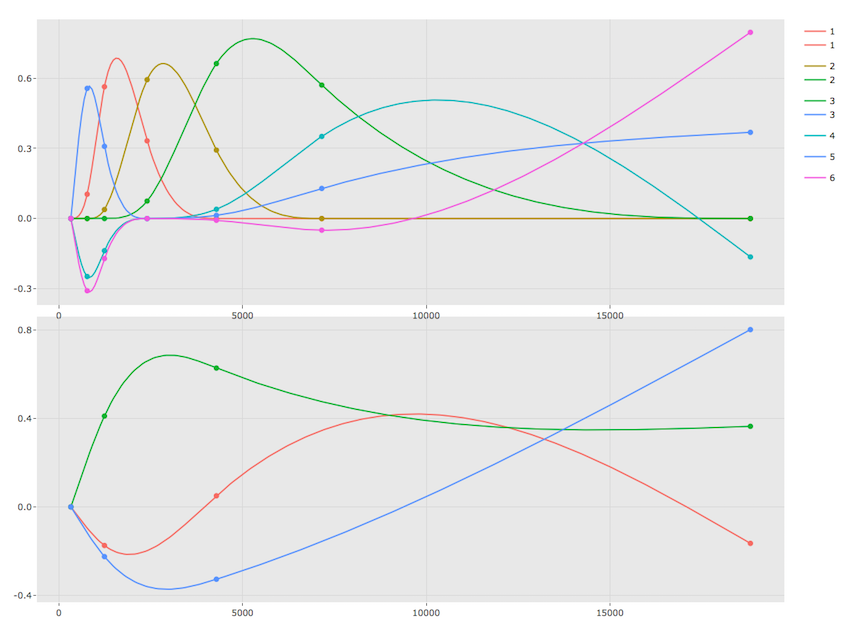
\includegraphics[width=145mm,scale=0.8]{images/splines_subplot.png}
  \caption{Multiple splines visualizations with different degree of freedom.}
  \label{figure:splines_subplot}
\end{figure}

\subsection{Illustrations}\label{illustrations}

There will likely be several sections, perhaps including code snippets,
such as:

\begin{Schunk}
\begin{Sinput}
autoplotly(prcomp(iris[c(1, 2, 3, 4)]), data = iris, frame = TRUE, colour = 'Species')
\end{Sinput}
\end{Schunk}

\begin{figure}[htbp]
  \centering
  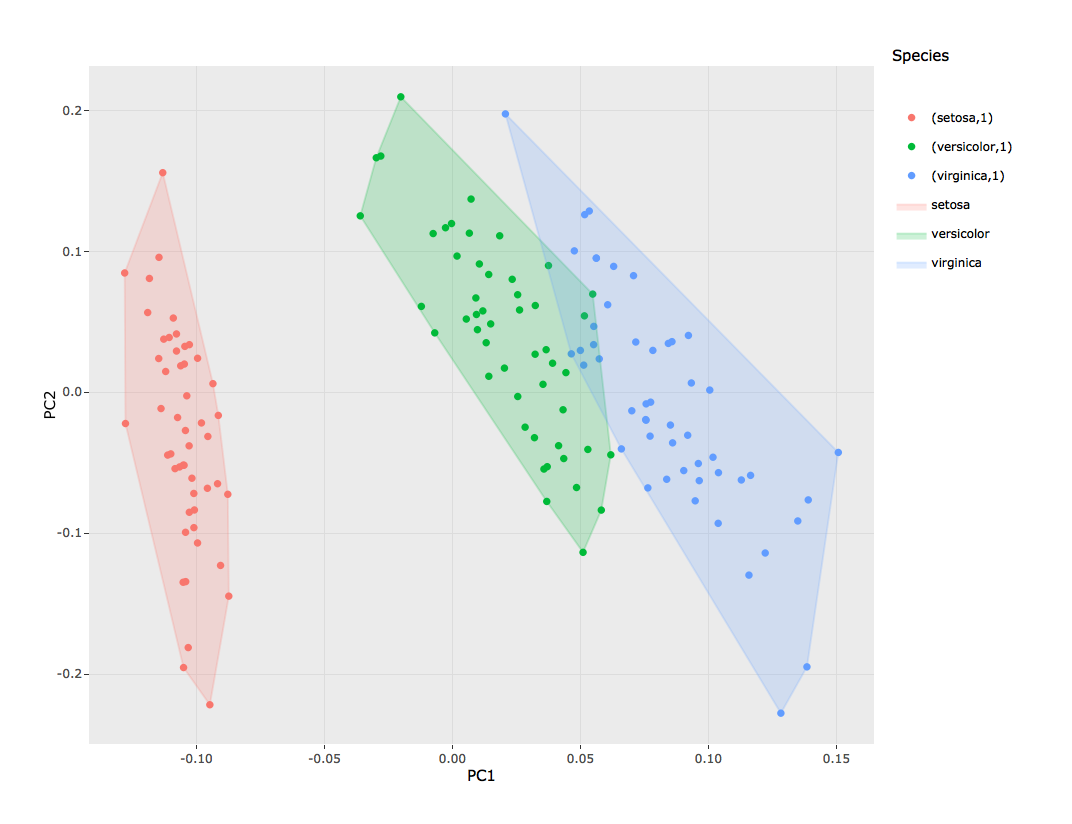
\includegraphics[width=145mm,scale=0.8]{images/iris_pca_full.png}
  \caption{PCA with clolors and boundary for each class.}
  \label{figure:pca_full}
\end{figure}

Forecasting packages such as \CRANpkg{forecast} \citep{forecast},
\CRANpkg{changepoint} \citep{changepoint}, \CRANpkg{strucchange}
\citep{strucchange}, and \CRANpkg{dlm} \citep{dlm}, are popular choices
for statisticians and researchers. Interactive visualizations of
predictions and statistical results from those packages can be generated
automatically using the functions provided by \pkg{autoplotly} with the
help of \pkg{ggfortify}.

The \pkg{autoplotly} function automatically plots the change points with
optimal positioning for the \code{AirPassengers} data set found in the
\pkg{changepoint} package using the \code{cpt.meanvar} function, shown
in Figure \ref{figure:changepoint_caption}.

\begin{Schunk}
\begin{Sinput}
library(changepoint)
autoplotly(cpt.meanvar(AirPassengers))
\end{Sinput}
\end{Schunk}

\begin{figure}[htbp]
  \centering
  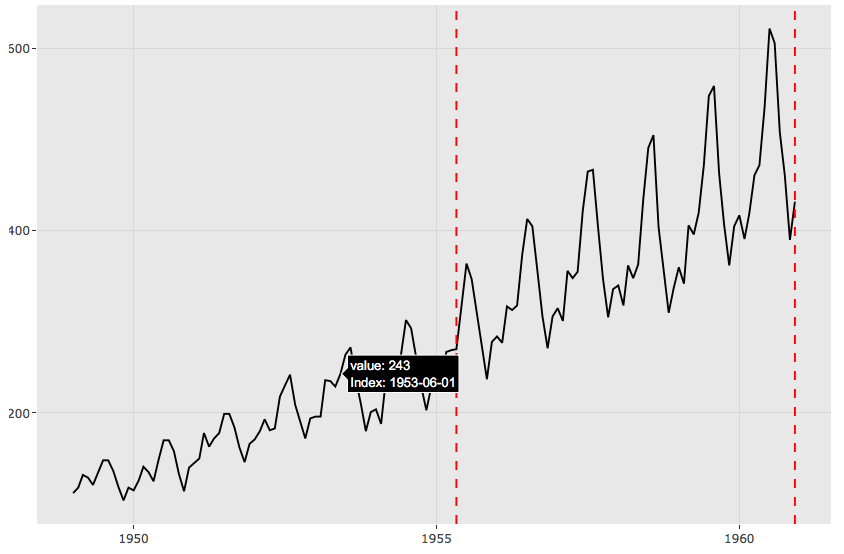
\includegraphics[width=145mm,scale=0.8]{images/changepoint_caption.png}
  \caption{Change points with optimal positioning for AirPassengers.}
  \label{figure:changepoint_caption}
\end{figure}

The \pkg{autoplotly} function automatically plots the original and
smoothed line from Kalman filter function in \pkg{dlm} package as shown
in Figure \ref{figure:dlm_caption}.

\begin{Schunk}
\begin{Sinput}
library(dlm)
form <- function(theta){
  dlmModPoly(order = 1, dV = exp(theta[1]), dW = exp(theta[2]))
}
model <- form(dlmMLE(Nile, parm = c(1, 1), form)$par)
filtered <- dlmFilter(Nile, model)
autoplotly(filtered)
\end{Sinput}
\end{Schunk}

\begin{figure}[htbp]
  \centering
  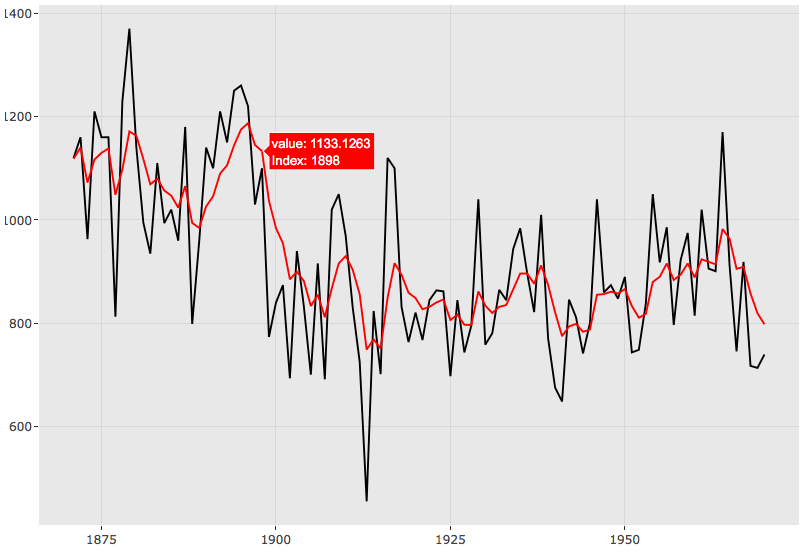
\includegraphics[width=145mm,scale=0.8]{images/dlm_caption.png}
  \caption{Smoothed time series by Kalman filter.}
  \label{figure:dlm_caption}
\end{figure}

Additionally, \pkg{autoplotly} plots the optimal break points where possible structural changes happen in the regression models built by the \code{strucchange::breakpoints}, shown in Figure \ref{figure:strucchange_caption}.

\begin{Schunk}
\begin{Sinput}
library(strucchange)
autoplotly(breakpoints(Nile ~ 1), ts.colour = "blue", ts.linetype = "dashed",
           cpt.colour = "dodgerblue3", cpt.linetype = "solid")
\end{Sinput}
\end{Schunk}

\begin{figure}[htbp]
  \centering
  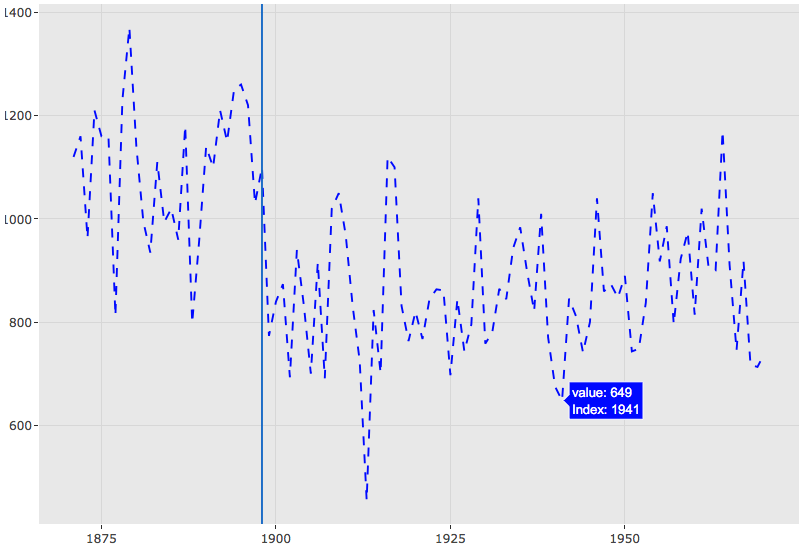
\includegraphics[width=145mm,scale=0.8]{images/strucchange_caption.png}
  \caption{Optimal break points with possible structural changes.}
  \label{figure:strucchange_caption}
\end{figure}


The \code{autoplotly} can also automatically generate interactive plots for results producuced by \pkg{splines}, shown in Figure \ref{figure:splines_caption}

\begin{Schunk}
\begin{Sinput}
library(splines)
autoplotly(ns(diamonds$price, df = 6))
\end{Sinput}
\end{Schunk}

\begin{figure}[htbp]
  \centering
  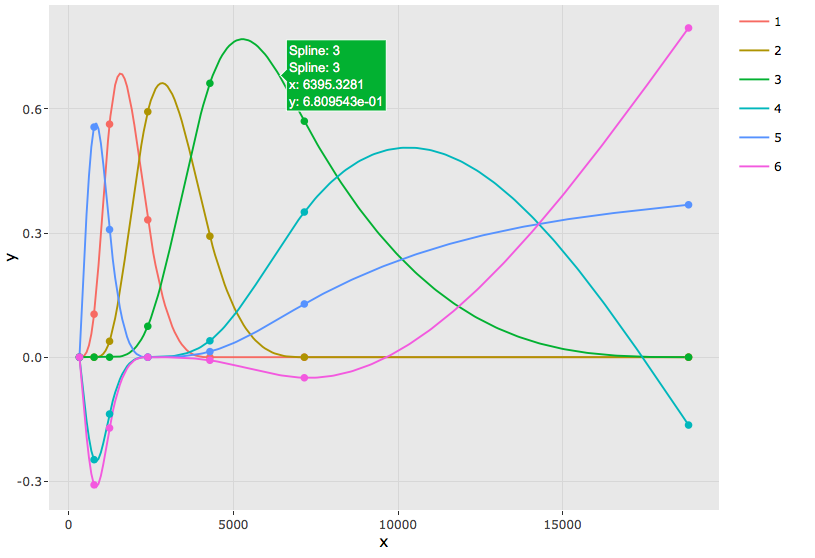
\includegraphics[width=145mm,scale=0.8]{images/splines_caption.png}
  \caption{B-spline basis points for natural cubic spline with boundary knots.}
  \label{figure:splines_caption}
\end{figure}

\subsection{Summary}\label{summary}

This file is only a basic article template. For full details of
\emph{The R Journal} style and information on how to prepare your
article for submission, see the
\href{https://journal.r-project.org/share/author-guide.pdf}{Instructions
for Authors}. \bibliography{RJreferences}

\address{%
Yuan Tang\\
H2O.ai\\
2309 Wake Robin Drive\\ West Lafayette, IN 47906\\
}
\href{mailto:terrytangyuan@gmail.com}{\nolinkurl{terrytangyuan@gmail.com}}

